\section{Bakgrund}

Projektet började våren 2013 som ett internt verktyg på Developer's Helsinki efter ett behov uppstått för ett system som skulle tillåta snabb implementering av personaliserat innehåll på kunders webbsidor.

Eftersom det i den tiden inte fanns någon färdig implementation att använda, bestämmdes det att det skulle uvecklas en mjukvara först för internt bruk men med målsättningen att lanseras som en SaaS produkt.

\subsection{Anpassat innehåll}

\begin{figure}[h!]
\centering
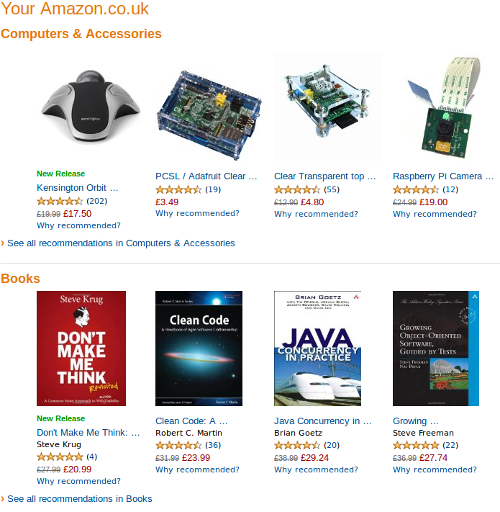
\includegraphics[width=120mm]{assets/images/amazon.png}
\caption{Amazons användarsida med anpassat innehåll}
\label{overflow}
\end{figure}

Anpassat innehåll, eller personaliserat innehåll (eng. \textit{Personalized content}), är innehåll som väljs ut på basis av egenskaper hos användaren. I fallet av webbsidor kan det handla om information som användarens geografiska läge, användarens språk, användarens webbläsare, antalet besök som användaren gjort till sidan, med mera.

Anpassat innehåll har bland annat användts inom nätburiker för att visa reklam anpassad för kunden på basis av dennes bäställningshistorik, bilden \ref{overflow} visar användarsidan som visas då man loggar in på amazons webb-butik. Inom social media har används anpassat innehåll för att lyfta fram innehåll som antas vara intressant för användaren (Uppdateringar från vänner som användaren ofta är i kontakt med, reklam från företag användaren har gillat m.m.).


\subsection{Behov}

I takt med att stora aktörer mer och mer förlitar sig på anpassat innehåll blir det allt mer atraherande för mindre webbsidor att använda sig av liknande teknik.

Allt flere användargränssnitt innehåller dels manuell och dels automatisk organisering av innehåll, så väl på webben som på terminaler som datorer och mobila enheter.

\subsection{Befinttliga lösningar}

Lösningar som redan skapats, undersök om det finns nåt att lära sig.



% vim: set tw=78:ts=2:sw=2:et:fdm=marker:wrap:wm=78:ft=tex
% vim: spell spelllang=sv
